\chapter{Physics}

	\section{Collision Box}
	Each collision box have four points: upper--left, upper--right, lower--left and lower--right. This points represents the translated points: the points are created accordling to Sprite coordinates, but the collision is computed using the translated points (computed from the Character position). In the Character collision detection the actual Sprite must have its collision boxes translated to the actual Character position.
	\begin{figure}[H]
		\centering
		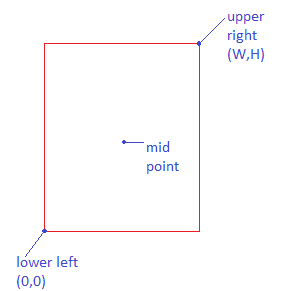
\includegraphics[]{img/collisionboxcoordinates.png}
		\caption{Collision Box coordinates Accordling to the Sprite coordinates. }
		\label{fig:collisionBox}
		
	\end{figure}